%\documentclass{book}\usepackage{sjtfonts}\usepackage{includegraphics}\usepackage{alltt}\usepackage{latexsym}
%\usepackage{array}
%\begin{document}\input{defs0}%		miradefs.tex 		    June 1994

% opening and closing a quoted Miranda section

\newcommand{\mira}{\noindent\hrulefill\nopagebreak\so}
\newcommand{\arim}{\nopagebreak\st\hrulefill\\}

% backslash in the Miranda environment
% Only feasible approach is to use \verb+\+
% in line!

%\newcommand{\bs}{$\mi\backslash\!\!$}
%\newcommand{\lbs}{\mbox{\verb+\+}}

% ignoring part of the input

\newcommand{\ignore}[1]{}

% a blank line in a Miranda section

\newcommand{\bl}{\mbox{\ }}

% Signalling a diffculty.

\definecolor{light-gray}{gray}{0.95}

\newcommand{\beware}[2]
 {\medskip\noindent\colorbox{light-gray}{\parbox{\textwidth}
 {\mbox{\large\textbf{#1}} \medskip\noindent\\ #2}\medskip\noindent}}

% Subscripting in Miranda text
\newcommand{\subscr}[2]{\mbox{${\mbox{\texttt{#1}}}_{\mbox{\texttt{#2}}}$}}

%\newcommand{\subscr}[2]{\mbox{${\mbox{\mi #1}}_{\mbox{\smtt #2}}$}}
\newcommand{\aone}{\subscr{a}{1}}
\newcommand{\atwo}{\subscr{a}{2}}
\newcommand{\ak}{\subscr{a}{k}}

\newcommand{\aoneone}{\subscr{a}{1,1}}

\newcommand{\eone}{\subscr{e}{1}}
\newcommand{\etwo}{\subscr{e}{2}}
\newcommand{\ei}{\subscr{e}{i}}
\newcommand{\er}{\subscr{e}{r}}

\newcommand{\fone}{\subscr{f}{1}}
\newcommand{\fl}{\subscr{f}{l}}

\newcommand{\gone}{\subscr{g}{1}}
\newcommand{\gtwo}{\subscr{g}{2}}
\newcommand{\gi}{\subscr{g}{i}}
\newcommand{\gr}{\subscr{g}{r}}

\newcommand{\hone}{\subscr{h}{1}}
\newcommand{\hl}{\subscr{h}{l}}

\newcommand{\pone}{\subscr{p}{1}}
\newcommand{\ptwo}{\subscr{p}{2}}
\newcommand{\pk}{\subscr{p}{k}}

\newcommand{\qone}{\subscr{q}{1}}
\newcommand{\qtwo}{\subscr{q}{2}}
\newcommand{\qk}{\subscr{q}{k}}

\newcommand{\rone}{\subscr{r}{1}}
\newcommand{\rtwo}{\subscr{r}{2}}

\newcommand{\tone}{\subscr{t}{1}}
\newcommand{\ttwo}{\subscr{t}{2}}
\newcommand{\tn}{\subscr{t}{n}}

\newcommand{\vone}{\subscr{v}{1}}
\newcommand{\vtwo}{\subscr{v}{2}}
\newcommand{\vn}{\subscr{v}{n}}

% for regular expressions

\newcommand{\stone}{\subscr{st}{1}}
\newcommand{\sttwo}{\subscr{st}{2}}
\newcommand{\stn}{\subscr{st}{n}}
\newcommand{\rthree}{\subscr{r}{3}}

\newcommand{\eps}{$\varepsilon$}
\newcommand{\trans}[1]{\stackrel{\mbox{\tt #1}}{\longrightarrow}}



% superscript in Miranda text

\newcommand{\superscr}[2]{\mbox{${\mbox{\mi #1}}^{\mbox{\smtt #2}}$}}

% Not equals in Miranda text

\newcommand{\noteq}{\makebox[0pt][l]{=}/}
\newcommand{\overslash}{\makebox[0pt][l]{/}}

% Definitions in complexity chapter

\newfont{\oldSym}{cmsy10}
\newcommand{\Th}{\boldmath$\oldSym\Theta$}
\newcommand{\pow}[1]{\^{}#1}
\newcommand{\leqq}{$\leq$}
\newcommand{\geqq}{$\geq$}
\newcommand{\lll}{$\ll$}
\newcommand{\eqq}{$\equiv$}
\newcommand{\ltwo}{\subscr{log}{2}}

% Indexing

\newcommand{\minx}[1]{\index{#1@{\ttfamily{}#1}}}


\chapter{Data types, tuples and lists}
\chapstart
\label{tupleList}

Thus far we have looked at programs which work over the basic types \texttt{Integer}, \texttt{Int}, \texttt{Float}, \texttt{Bool} and \texttt{Char}, and we have also seen how to design enumerated types like the \texttt{Move} type in the Rock - Paper - Scissors game. We've also looked at strategies for designing programs in general, including breaking problems down into smaller problems to solve them in steps.
However, in practical problems we will want to represent more complex things, 
as we saw with our \texttt{Picture} example 
in Chapter \ref{intro}.

This chapter introduces two ways of building compound data built into Haskell; these are the \textbf{tuple} and the \textbf{list}, and in particular the \texttt{String} type. We'll also look again at ways of defining \texttt{data} types for ourselves. Together they are enough
to let us represent many different kinds of `structured' information.
We shall meet other ways of defining data types for ourselves 
in Chapters \ref{algTypes} and \ref{adt}. 

After looking at these various types, we'll explain how to manipulate tuples and lists, and in particular we introduce the `list
comprehension' notation to write down descriptions of how lists may be formed 
from other lists, and use this in a database case study. 

In the chapters to come we look at the range of built-in list processing functions, aw well as how list-manipulating functions can be defined from scratch.

\section{Introducing tuples and lists}
\index{tuples!and lists}

Both tuples and lists are built up by combining a number of pieces of data 
into a single object, but they have different properties. 
\begin{itemize}
\item
In a tuple, we
combine a fixed number of values of fixed types -- which might be 
different --
into a single object. 
\item
In a list we combine an arbitrary number of values
-- all of the same type -- into a single object. 
\end{itemize}
Let's look at an example to clarify the 
difference. Suppose that we want to
make a simple model of a supermarket, and as part of that model
we want to record the contents of someone's shopping basket.

\subsubsection*{Individual items}

A given item has a name and a price (in pence), and we therefore need somehow to 
combine these two pieces of information. We do this in a tuple,
such as
\begin{alltt}
("Salt:\ 1kg",139)
("Plain crisps",25)
\end{alltt}
where in each tuple a \texttt{String} is combined with an \texttt{Int}.
\begin{itemize}
\item
The \texttt{String} gives the name of the item.
\item
The \texttt{Int} gives its price, in pence.\footnote{We use an \texttt{Int} here rather than an \texttt{Integer} because we can be sure that prices of individual items, and also totals for shopping bills, will always be `small' integers.}
\end{itemize}
We can give names to types in Haskell, so that types are made easier to
read, and we name this \textbf{tuple type} \texttt{ShopItem} like this:
\begin{alltt}\minx{type}
type ShopItem = (String,Int)\minx{ShopItem}
\end{alltt}
Now we can say that `\texttt{("Salt:\ 1kg",139)} is a \texttt{ShopItem}' or
\begin{alltt}
("Salt:\ 1kg",139) ::\ ShopItem
\end{alltt}

\subsubsection*{The shopping basket}

\noindent
How are the contents of the basket represented? We know that we have a collection
of items, but we do not know in advance how many we have; one basket might contain
ten items, another one three; a third might be empty. Each item is represented in the same way,
as a member of the \texttt{ShopItem} type, and so we represent the
contents of the basket by a \textbf{list} of these, as in the list
\begin{alltt}
[ ("Salt:\ 1kg",139) , ("Plain crisps",25) , ("Gin:\ 1lt",1099) ]
\end{alltt}
This is a member of the \textbf{list type}
\begin{alltt}
[ (String,Int) ]
\end{alltt}
which we can also write
\begin{alltt}
[ ShopItem ]
\end{alltt}
Other members of this list type include the empty list, \texttt{[]},\minx{[]} and
the basket above with a second packet of crisps replacing the gin:
\begin{alltt}
[ ("Salt:\ 1kg",139) , ("Plain crisps",25) , ("Plain crisps",25) ]
\end{alltt}
We can give a name to this type too:
\begin{alltt}\minx{type}
type Basket   = [ShopItem]\minx{Basket}
\end{alltt}

\beware{Tuples, lists and type checking}{\index{type checking!tuples and lists}
Every member of the \texttt{ShopItem} type will have two components -- a \texttt{String}
and an \texttt{Int} -- as specified in the type
\texttt{(String,Int)}. If we are given a member of this type we can
therefore predict what type its components will have, and this means that we can 
check that these components are used in an appropriate way: we can check
that we deal with the second half as an \texttt{Int} and not a
\texttt{Bool}, for example. 

\medskip
Turning to the \texttt{Basket} type, since every member of the list has the same type, we can predict
the type of any item chosen from the list: it will be a \texttt{ShopItem}. 

\medskip
Suppose instead that Haskell allowed lists whose
members could have different types: if we choose the first element of
such a list we cannot predict its type, and so we lose the ability to
type-check programs before they are run. Because we want to keep this
important property, Haskell is designed so that lists
have to contain elements of the same type, but different lists will
contain elements of different types.

\medskip
We therefore keep the property, first
mentioned in Chapter \ref{intro}, that we can type-check \index{type-checking}
all programs prior
to execution, and so any type errors in a program can
be found before a program is actually executed.


}

\beware{Naming types}{
As we have seen, we can give names to types in Haskell, as in the definition
\begin{alltt}
type ShopItem = (String,Int)
\end{alltt}
The keyword \texttt{type}\minx{type} introduces the fact that this
is the definition of a type rather than a value. We can also tell this
because the type names \texttt{ShopItem} and \texttt{Basket} begin with
capital letters, as noted in Section \ref{syntax}. Built into the system is the definition
\begin{alltt}\minx{String}
type String = [Char]\minx{String}
\end{alltt}
so Haskell treats strings as a special case of the list type. Names such
as \texttt{ShopItem} and \texttt{String} are \textbf{synonyms}\index{synonym}
for the types which they name.

\medskip
\noindent
A \texttt{type}\minx{type} definition like this is treated as shorthand in Haskell -- wherever a name
like \texttt{ShopItem} is used, it has exactly the same effect as if {\mi
(String,Int)} had been written. Definitions like this make programs
more readable and also lead to more comprehensible type error
messages.
}

\medskip\noindent
We now look at tuple types in more detail, and examine some examples of
how tuples are used in practice.

\section{Tuple types}
\index{tuples|(}

The last section introduced the idea of tuple types. In general a tuple
type is 
built up from components of simpler types. The type
\begin{alltt}
(\tone,\ttwo,\ldots,\tn)
\end{alltt}
consists of tuples of values
\begin{alltt}
(\vone,\vtwo,\ldots,\vn)
\end{alltt}
in which \texttt{\vone ::\tone}, \ldots, \texttt{\vn ::\tn}. In other words, each
component \texttt{\subscr{v}{i}} of the tuple has to have the type  
\texttt{\subscr{t}{i}} given in the corresponding position 
in the tuple type. 


The reason for the name `tuple' is that these objects are usually called pairs,
triples, quadruples, quintuples, sextuples and so on. The general word for
them is therefore `tuple'. In other programming languages, these types are
called records or structures; see Appendix \ref{vs} for a more detailed
comparison. 

We can model a type of supermarket items by the \texttt{ShopItem} type
defined by
\begin{alltt}
type ShopItem = (String,Int)
\end{alltt}
and we saw above that its members include items like \texttt{("Gin,
1lt",1099)}.
How else are tuple types used in programs? We look at a series of examples now.


\begin{example}
\subexample*{1.} 
First, we can use a tuple to return
a compound result from a function, as in the example where we are
required to return both the minimum and the maximum of two \texttt{Integers}
\begin{alltt}
minAndMax :: Integer -> Integer -> (Integer,Integer)\minx{minAndMax}
minAndMax x y
  | x>=y        = (y,x)
  | otherwise   = (x,y)
\end{alltt}

\subexample*{2.} 
Secondly, suppose we are asked to find a (numerical) solution to a problem when it is 
uncertain whether
a solution actually exists in every case: this might be the question of where a straight line meets
the horizontal or x-axis, for instance.  
\begin{center}
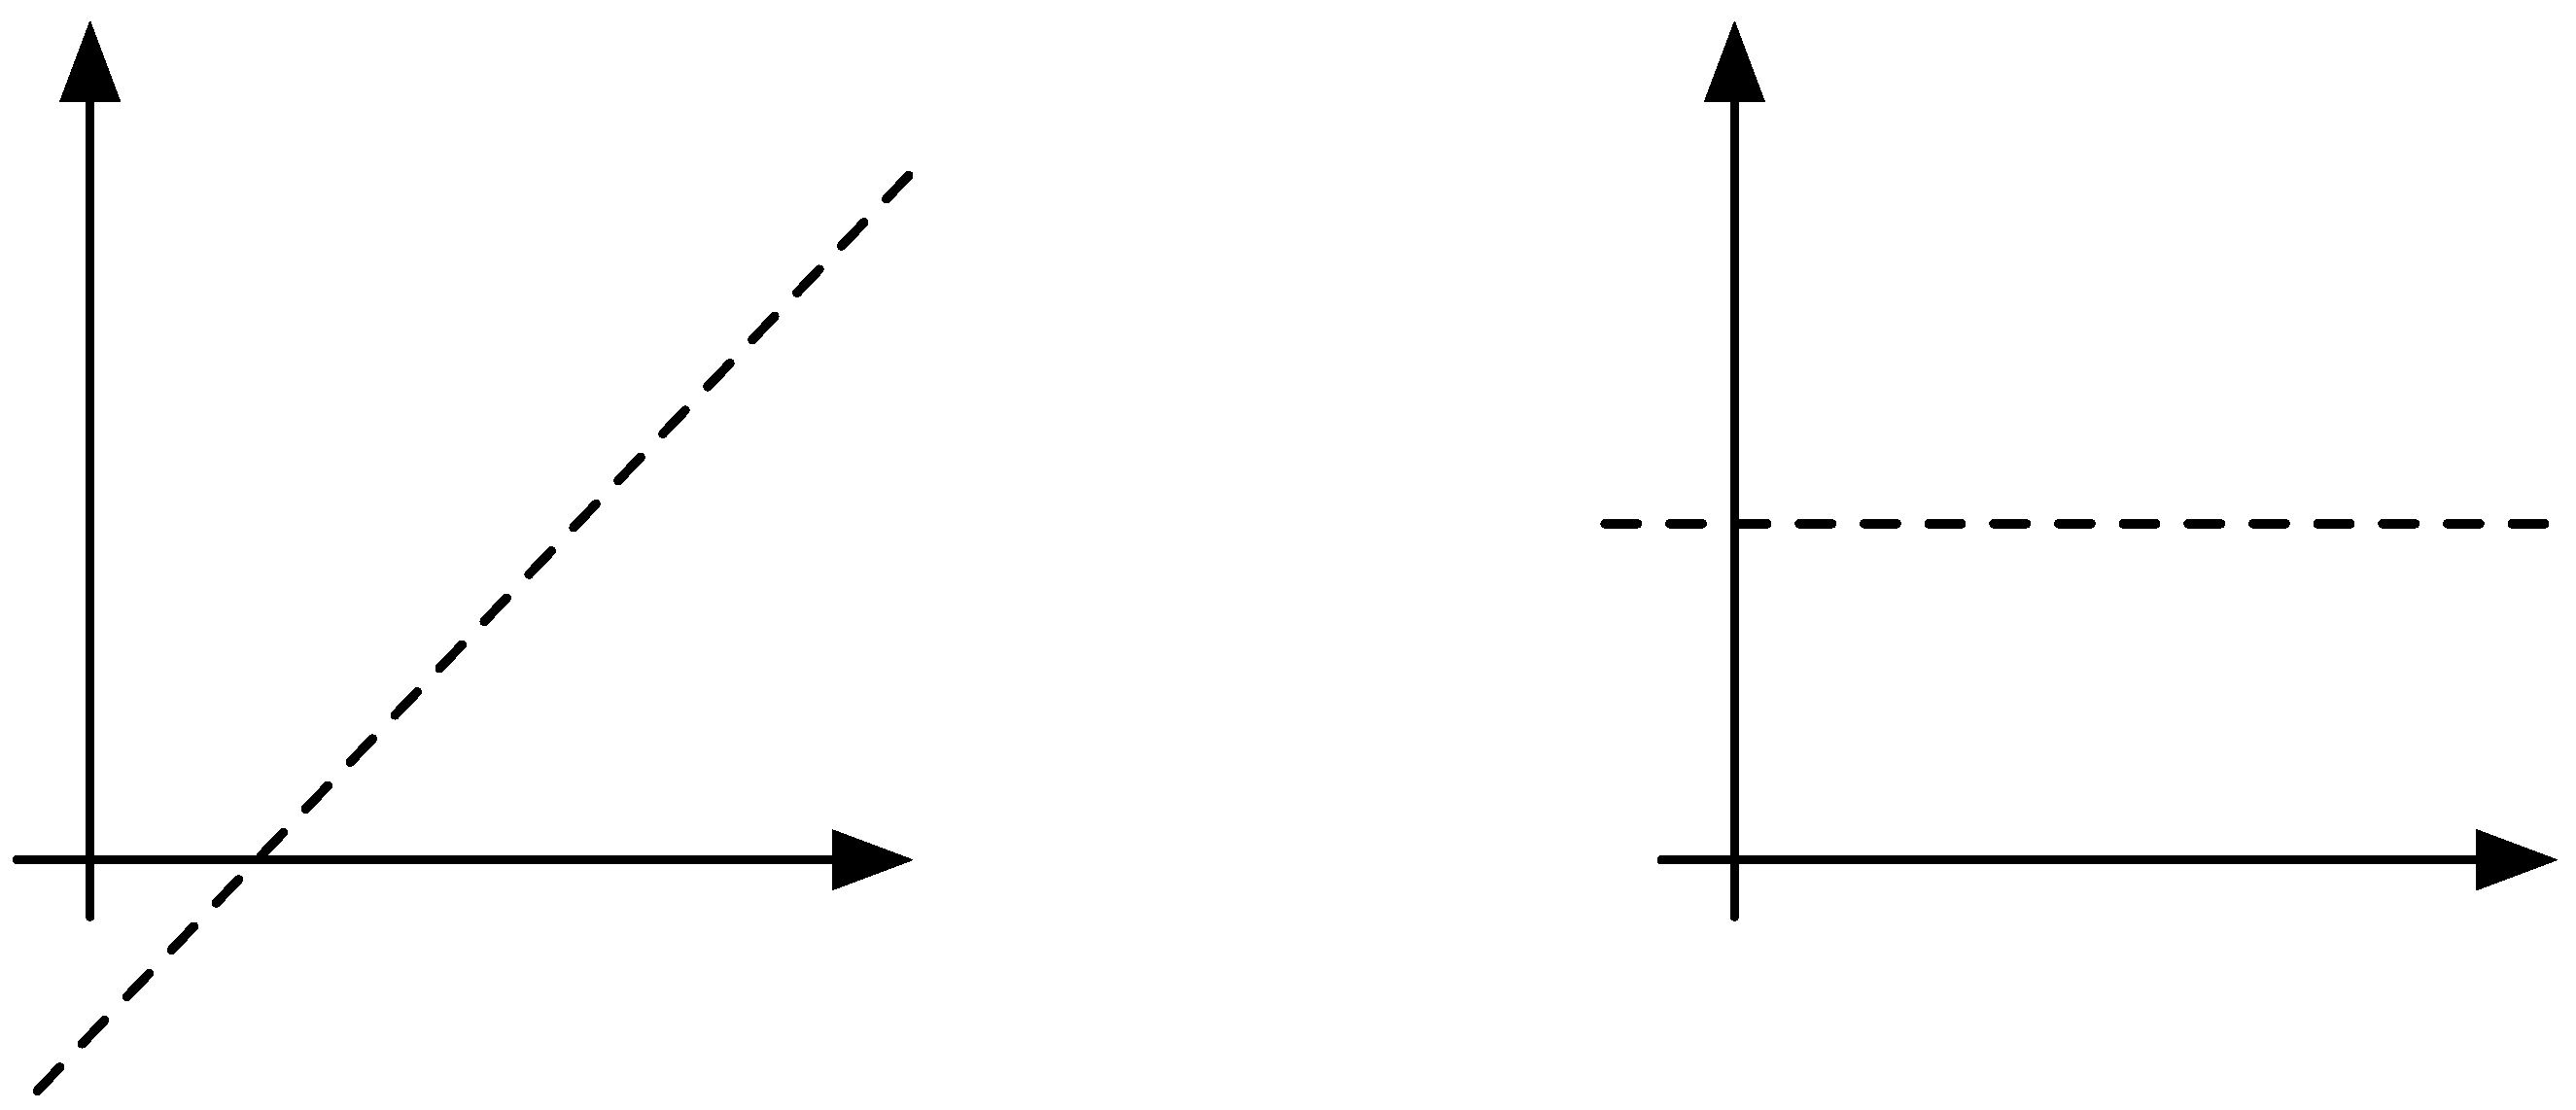
\includegraphics[width=3in]{Pictures/lineSoln.pdf}
\end{center}
One way of dealing with this is for the
function to return a \texttt{(Float,Bool)} pair. If the boolean part is {\mi
False}, this signals that no solution was found; if it is like {\mi
(2.1,True)}, it indicates that \texttt{2.1} is indeed the solution.
\end{example}

\subsection*{Pattern matching}

Next we turn to look at how functions can be defined over tuples.
Functions over tuples are usually defined by \textbf{pattern matching}\index{pattern matching}.
Instead of writing
a variable for an argument of type \texttt{(Integer,Integer)}, say, a \textbf{pattern},
\index{pattern}
\texttt{(x,y)}
is used. 
\begin{alltt}
addPair :: (Integer,Integer) -> Integer\minx{addPair}
addPair (x,y) = x+y
\end{alltt}
On application the components of the pattern
are matched by the corresponding components of the argument, so that on
applying the function \texttt{addPair} to the argument \texttt{(5,8)}
the value \texttt{5} is matched to \texttt{x}, and \texttt{8} to
\texttt{y}, giving the calculation
\begin{alltt}
addPair (5,8) 
\step 5+8
\step 13
\end{alltt}
Patterns can contain literals and nested patterns,\index{pattern!nested}
as in the examples
\begin{alltt}
addPair (0,y) = y
addPair (x,y) = x+y

shift :: ((Integer,Integer),Integer) -> (Integer,(Integer,Integer))
shift ((x,y),z) = (x,(y,z))
\end{alltt}
Functions which pick out particular parts of a tuple can be defined by
pattern matching. For the \texttt{ShopItem} type, the definitions might be
\begin{alltt}
name  :: ShopItem -> String
price :: ShopItem -> Int

name  (n,p) = n
price (n,p) = p
\end{alltt}
Haskell has these \textbf{selector functions} on pairs built in. They are
\index{selector}\index{function!selector}
\begin{alltt}
fst (x,y) = x\minx{fst}
snd (x,y) = y\minx{snd}
\end{alltt}
Given these selector functions we can avoid pattern matching if
we so wish. For instance, we could redefine \texttt{addPair} like this
\begin{alltt}
addPair :: (Integer,Integer) -> Integer\minx{addPair}
addPair p = fst p + snd p
\end{alltt}
but generally a pattern-matching definition is easier to read than
one which uses selector functions instead.


\begin{example}
\subexample*{3.} 
We first introduced the Fibonacci numbers\index{Fibonacci numbers} 
\begin{alltt}
0, 1, 1, 2, 3, 5, ... , u, v, (u+v), ...
\end{alltt}
in Section \ref{genRecursion}, where we gave an inefficient recursive definition of
the sequence. Using a tuple we can give an efficient
solution to the problem. The next value in the sequence is given by
adding the previous two, so what we do is to write a function which
returns {\em two consecutive values\/} as a result. In other words we want to define
a function \texttt{fibPair} so that it has the property that
\begin{alltt}
fibPair n = (fib n , fib (n+1))
\end{alltt} 
then given such a pair, \texttt{(u,v)} we get the next pair as
\texttt{(v,u+v)}, which is exactly the effect of the \texttt{fibStep} function:
\begin{alltt}
fibStep :: (Integer,Integer) -> (Integer,Integer)\minx{fibStep}
fibStep (u,v) = (v,u+v)
\end{alltt}
This gives us the definition of the `Fibonacci pair' function
\begin{alltt}
fibPair :: Integer -> (Integer,Integer)\minx{fibPair}
fibPair n
  | n==0        = (0,1)
  | otherwise   = fibStep (fibPair (n-1))
\end{alltt}
and we can define
\begin{alltt}
fastFib :: Integer -> Integer\minx{fastFib}
fastFib = fst . fibPair
\end{alltt}
where recall that `\texttt{.}'\minx{.} composes the two functions, passing the
output of \texttt{fibPair}
to the input of \texttt{fst}, which picks out its first component.
\end{example}

\beware{One pair or two arguments?}{\index{pitfalls!paired arguments}\index{argument!tuple}
It is important to distinguish between the functions\minx{fibStep}\minx{fibTwoStep}
\begin{alltt}
fibStep :: (Integer,Integer) -> (Integer,Integer)\\
fibStep (x,y) = (y,x+y)\\
\ \\
fibTwoStep :: Integer -> Integer -> (Integer,Integer)\\
fibTwoStep x y = (y,x+y)
\end{alltt}
\texttt{fibStep} has a single argument which is a pair of numbers,
while \texttt{fibTwoStep} has two arguments, each of which is
a number. We shall see later that the second function
can be used in a more flexible way than the first; for the moment it is
important to realize that there is a difference, and that type errors will
result if we confuse the two and write\index{type error}
\begin{alltt}
fibStep 2 3\ \ \ \ \ \ \ \ \ \ \ \ \ \ \ \ \ \ \ \ \ fibTwoStep (2,3)
\end{alltt}
We say more about the relationship between these two functions in Section
\ref{curry}.
}

\begin{exercises}
\item
Give a definition of the function
\begin{alltt}
maxOccurs :: Integer -> Integer -> (Integer,Integer)
\end{alltt}
which returns the maximum of two integers, together with the number of times
it occurs. Using this, or otherwise, define the function
\begin{alltt}
maxThreeOccurs :: Integer -> Integer -> Integer -> (Integer,Integer)
\end{alltt}
which does a similar thing for three arguments.

\item
Give a definition of a function
\begin{alltt}
orderTriple :: (Integer,Integer,Integer) -> (Integer,Integer,Integer)
\end{alltt} 
which puts the elements of a triple of three integers into ascending order.
You might like to use the \texttt{maxThree}, \texttt{middle} and
\texttt{minThree} functions defined earlier.

\item
Define the function which finds where a straight line crosses the x-axis. 
You will need to think about how to supply the information about the
straight line to the function.

\item Design test data for the preceding exercises; explain the choices you
have made in each case. Give a sample evaluation of each of your functions.
\index{tuples|)}

\end{exercises}



\section{Introducing algebraic types}
\label{introAlg}\index{type!algebraic|see{algebraic type}}\index{algebraic type|(}

We have already seen that it's useful to be able to define our own enumerated types, such as a move in the Rock - Paper - Scissors game, a day of the week, or a season of the year. In this section we'll see that we can use \texttt{data} types for much more general combinations of values. 


Algebraic data type definitions are introduced by the keyword \texttt{data}, followed by 
the name of the type, an equals sign and then information about how elements are constructed by applying 
\textbf{constructors}.\index{constructor}  The names of the type and the constructors begin with
capital letters.

We give a sequence of examples of increasing complexity, first recapping enumerated types, then looking at single constructor product types, and finally looking at types which contain a number of alternative `shapes' of data. We look again at \texttt{data} types in Chapter \ref{algTypes}.

\subsection*{Enumerated types}
\index{enumerated type}

We have already seen examples of this, such as the type modelling a move in the Rock - Paper - Scissors game, in Section \ref{EnumTypes}. Recall that the definition lists the elements of the type, thus: 
\begin{alltt}
data Move = Rock | Paper | Scissors \minx{Move}
            deriving (Eq,Show)
\end{alltt}
and we can define functions by pattern matching over the values, as in
\begin{alltt}\minx{score}
score :: Move -> Move -> Integer
score Rock Rock     = 0
score Rock Paper    = -1
score Rock Scissors = 1
score Paper Rock    = 1
\end{alltt}
As we noted in Section \ref{EnumTypes} we can derive definitions of functions like equality using a `\texttt{deriving}' clause in the definition of a \texttt{data} type so that we don't need to define these functions for ourselves when we introduce a new data type definition. We will talk about the details of what underlies this in Section \ref{algClasses}.
 
 
\subsection*{Product types}
\index{product type}

Instead of using a tuple we can define a \texttt{data} type with a number of
components or fields, often called a \textbf{product} type. An
example might be
\begin{alltt}\minx{Person}\minx{People}
data People = Person Name Age \hfill (People)
              deriving (Eq,Show)
\end{alltt}
where \texttt{Name} is a synonym for \texttt{String}, and \texttt{Age} for \texttt{Int},
written thus:
\begin{alltt}
type Name = String
type Age  = Int
\end{alltt}
The definition of \texttt{People} should be read as saying
\[
\parbox{28pc}{To construct an element of type \texttt{People}, you need to supply two values;
one,
\texttt{st} say, of
type \texttt{Name}, and another, \texttt{n} say, of type \texttt{Age}. The
element of \texttt{People} formed from them will be \texttt{Person st n}.} 
\]
Example values of this type include\index{Jemima, Electric Aunt}
\begin{alltt}
Person "Electric Aunt Jemima" 77
Person "Ronnie" 14
\end{alltt}
As before,  
functions are defined using \textbf{pattern matching}. Any element of type 
\texttt{People} will have the form \texttt{Person st n}, and so we can use this pattern on the
left-hand side of a definition,
\begin{alltt}
showPerson :: People -> String
showPerson (Person st n) = st ++ " -- " ++ show n
\end{alltt}
(recall that \texttt{show} gives a textual form of an \texttt{Int}). For instance,\index{Jemima, Electric Aunt}
\index{Electric Aunt Jemima|see{Jemima, Electric Aunt}}
\begin{alltt}
showPerson (Person "Electric Aunt Jemima" 77)
 = "Electric Aunt Jemima -- 77"
\end{alltt}
Elements of the \texttt{People} type are made (or \texttt{constructed}) by applying the \textbf{constructor} \texttt{Person}. This is called a 
\textbf{binary} constructor
\index{constructor!binary}
because it takes two values to form a value of type 
\texttt{People}. For the enumerated types like \texttt{Move} the constructors
are called \textbf{nullary}
\index{constructor!nullary}
(or {\em 0-ary}) as they take no arguments. 
 
The constructors introduced by algebraic type definitions can be used
just like functions, so that \texttt{Person st n} is the result of applying
the function \texttt{Person} to the arguments \texttt{st} and \texttt{n}; we can
interpret the definition \texttt{(People)} as giving the \textbf{type of the constructor}, here
\begin{alltt}
Person :: Name -> Age -> People
\end{alltt}

\begin{figure}[t]
\beware{Tuples and \texttt{data} types}{\index{type!tuples and \texttt{data} types}
An alternative definition of the type of people is given by the type
synonym
\begin{alltt}
type People = (Name,Age)
\end{alltt}
The advantages of using an algebraic type are threefold.
\begin{titemize}\index{algebraic type!compared with tuple}
\index{tuples!compared with algebraic type}
\item Each object of the type carries an explicit \textbf{label} of the
purpose of the element; in this case that it represents a person.
\item It is not possible accidentally to treat an arbitrary pair consisting of
a string and a number as a person; a person must be constructed using the
\texttt{Person} constructor.
\item The type will appear
in any error messages due to mis-typing; a type synonym might be expanded out 
and so disappear from any type error messages.
\end{titemize} 
There are also advantages of using a tuple type, with a synonym declaration.
\begin{titemize}
\item The elements are more compact, and so definitions will be shorter.
\item Using a tuple, especially a pair, allows us to reuse many 
polymorphic functions such as \texttt{fst}, \texttt{snd} and
\texttt{unzip} over tuple types; this will not be the case for the
algebraic type.
\end{titemize}
In each system that
we model we will have to choose between these alternatives: our
decisions will depend exactly on how we use the products, and on the
complexity of the system.


The approach here works equally well with unary constructors, so we
\index{constructor!unary}
might say
\begin{alltt}
data Age = Years Int
\end{alltt}
whose elements are \texttt{Years 45} and so on. It is clear from a definition
like this that \texttt{45} is here being used as an age in years, rather than
some unrelated numerical quantity. The disadvantage is that we cannot use
functions defined over \texttt{Int} directly over \texttt{Age}.
}\end{figure}

\begin{figure}[t]
\beware{Type and constructor names}{\index{pitfalls!type and constructor names}
We can use the same name, for instance \texttt{Person}, for both the type and the
constructor of a type, as in the definition
\begin{alltt}
data Person = Person Name Age
\end{alltt}
We choose not to do this, as using the same name for two related but
different objects can easily lead to confusion, but it is an idiom used
by a number of Haskell programmers and in many Haskell libraries.
}\end{figure}
The examples of types given here are a special case of what we look at next.


\subsection*{Alternatives}
\index{algebraic type!alternatives}

A shape in a simple geometrical program is either a circle or a
rectangle. These alternatives are given by the type
\begin{alltt}\minx{Circle}\minx{Rectangle}
data Shape = Circle Float |\hfill(Shape)\minx{Shape}
             Rectangle Float Float
             deriving (Eq,Ord,Show)
\end{alltt}
which says that there are two ways of building an element of \texttt{Shape}. One
way is to supply the radius of a \texttt{Circle}; the other alternative is to give
the sides of a \texttt{Rectangle}. Example objects of this type are

\begin{alltt}
Circle 3.0
Rectangle 45.9 87.6
\end{alltt}
Pattern matching allows us to define functions by cases, as
in\index{algebraic type!pattern matching}
\index{pattern matching!algebraic type}
\begin{alltt}
isRound :: Shape -> Bool
isRound (Circle _)      = True
isRound (Rectangle _ _) = False
\end{alltt}
and also lets us use the 
components of the elements:
\begin{alltt}\label{areaDef}
area :: Shape -> Float
area (Circle r)      = pi*r*r
area (Rectangle h w) = h*w
\end{alltt}
Another way of reading the definition \texttt{(Shape)} is to say that
there are two \textbf{constructor functions} for the type \texttt{Shape}, whose
types are
\begin{alltt}
Circle    :: Float -> Shape
Rectangle :: Float -> Float -> Shape
\end{alltt}
These functions are called constructor functions because the elements of
the type are constructed by applying these functions.

Extensions of this type, to accommodate the position of an object, are
discussed in the exercises at the end of this section.

\subsection*{The general form of algebraic type definitions}
\index{algebraic type!general form}

The general form of the algebraic type definitions which we have seen so far is
\begin{alltt}
data Typename \hfill (Typename)
  = \subscr{Con}{1} \subscr{t}{11} \ldots \subscr{t}{1\subscr{k}{1}} | 
    \subscr{Con}{2} \subscr{t}{21} \ldots \subscr{t}{2\subscr{k}{2}} | 
        ....
    \subscr{Con}{n} \subscr{t}{n1} \ldots \subscr{t}{n\subscr{k}{n}}   
\end{alltt}
Each \texttt{\subscr{Con}{i}} is a constructor, followed by 
\subscr{k}{i}\ types, where \subscr{k}{i}\ is a non-negative integer which may
be zero. We build elements of the type \texttt{Typename} by applying these constructor
functions to arguments of the types given in the definition, so that
\begin{alltt}
\subscr{Con}{i} \subscr{v}{i1} \ldots \subscr{v}{i\subscr{k}{i}}
\end{alltt}
will be a member of the type \texttt{Typename} if \subscr{v}{ij} is 
in \subscr{t}{ij} for \texttt{j} ranging from \texttt{1} to \subscr{k}{i}. 

Reading the constructors as functions, the 
definition \texttt{(Typename)} gives the constructors the following
types
\begin{alltt}
\subscr{Con}{i} :: \subscr{t}{i1} -> \ldots -> \subscr{t}{i\subscr{k}{i}} -> Typename
\end{alltt}
In Chapter \ref{algTypes} we shall see two
extensions of the definitions seen already. 
\begin{titemize}
\item The types can be \textbf{recursive}\index{algebraic type!recursive|see{recursive type}};
we can use the type we are defining,
\texttt{Typename}, as (part of) any of the types \subscr{t}{ij}. This gives us
lists, trees and many other data structures.
\item The \texttt{Typename} can be followed by one or more type
variables which may be used on the right-hand side, making the definition
\textbf{polymorphic}. 
\end{titemize}
Recursive polymorphic types combine these two ideas, and this powerful
mixture provides types which can be reused in many different situations --
the built-in type of lists is an example of this kind of type. We look at these in Chapter \ref{algTypes}.

For the moment, however, we'll deal with the simple cases we have covered in this section, which are enough to model a wide variety of different problem domains, particularly in conjunction with tuples and lists.

\begin{figure}[t]
\beware{\texttt{type} and \texttt{data} definitions}{\index{pitfalls!\texttt{type} and \texttt{data}}
\index{type@\texttt{type} and \texttt{data}}Before we move on, it is worth contrasting \texttt{type} and \texttt{data} definitions.
A synonym given by \texttt{type} is simply a shorthand, and so a synonym type can always be
expanded out, and therefore removed from the program. 

\medskip
\noindent
On the other hand, a \texttt{data}
definition creates a new type. Because synonyms are simply shorthand, a
synonym definition cannot be recursive; \texttt{data} definitions can be
and often are recursive, as we shall discover in Chapter \ref{algTypes}.
}\end{figure}





\begin{exercises}


\item
Define a function to give the length of the perimeter of a geometrical shape,
of type \texttt{Shape}. What is the type of this function?

\item
Re-define the \texttt{Item} type for supermarket products so that it uses a \texttt{data} definition rather than a \texttt{type} definition.

\item
Add an extra constructor to \texttt{Shape} for triangles, and extend the
functions \texttt{isRound}, \texttt{area} and \texttt{perimeter} to include triangles.

\item
Define a function which decides whether a \texttt{Shape} is regular: a circle is
regular, a square is a regular rectangle and being equilateral makes a
triangle regular.

\item
Investigate the derived definitions for \texttt{Move} and \texttt{Shape}: what form
do the  \texttt{show} functions take, for example?

\item
Define an \texttt{==} function over \texttt{Shape} so that all circles of negative radius are
equated. How would you treat rectangles with negative sides?

\item
The type \texttt{Shape} takes no account of the position or orientation of a 
shape. After deciding how to represent points, how would you modify the
original definition of \texttt{Shape} to contain the \textbf{centre} of each object? You
can assume that rectangles lie with their sides parallel to the axes, thus:
\begin{center}
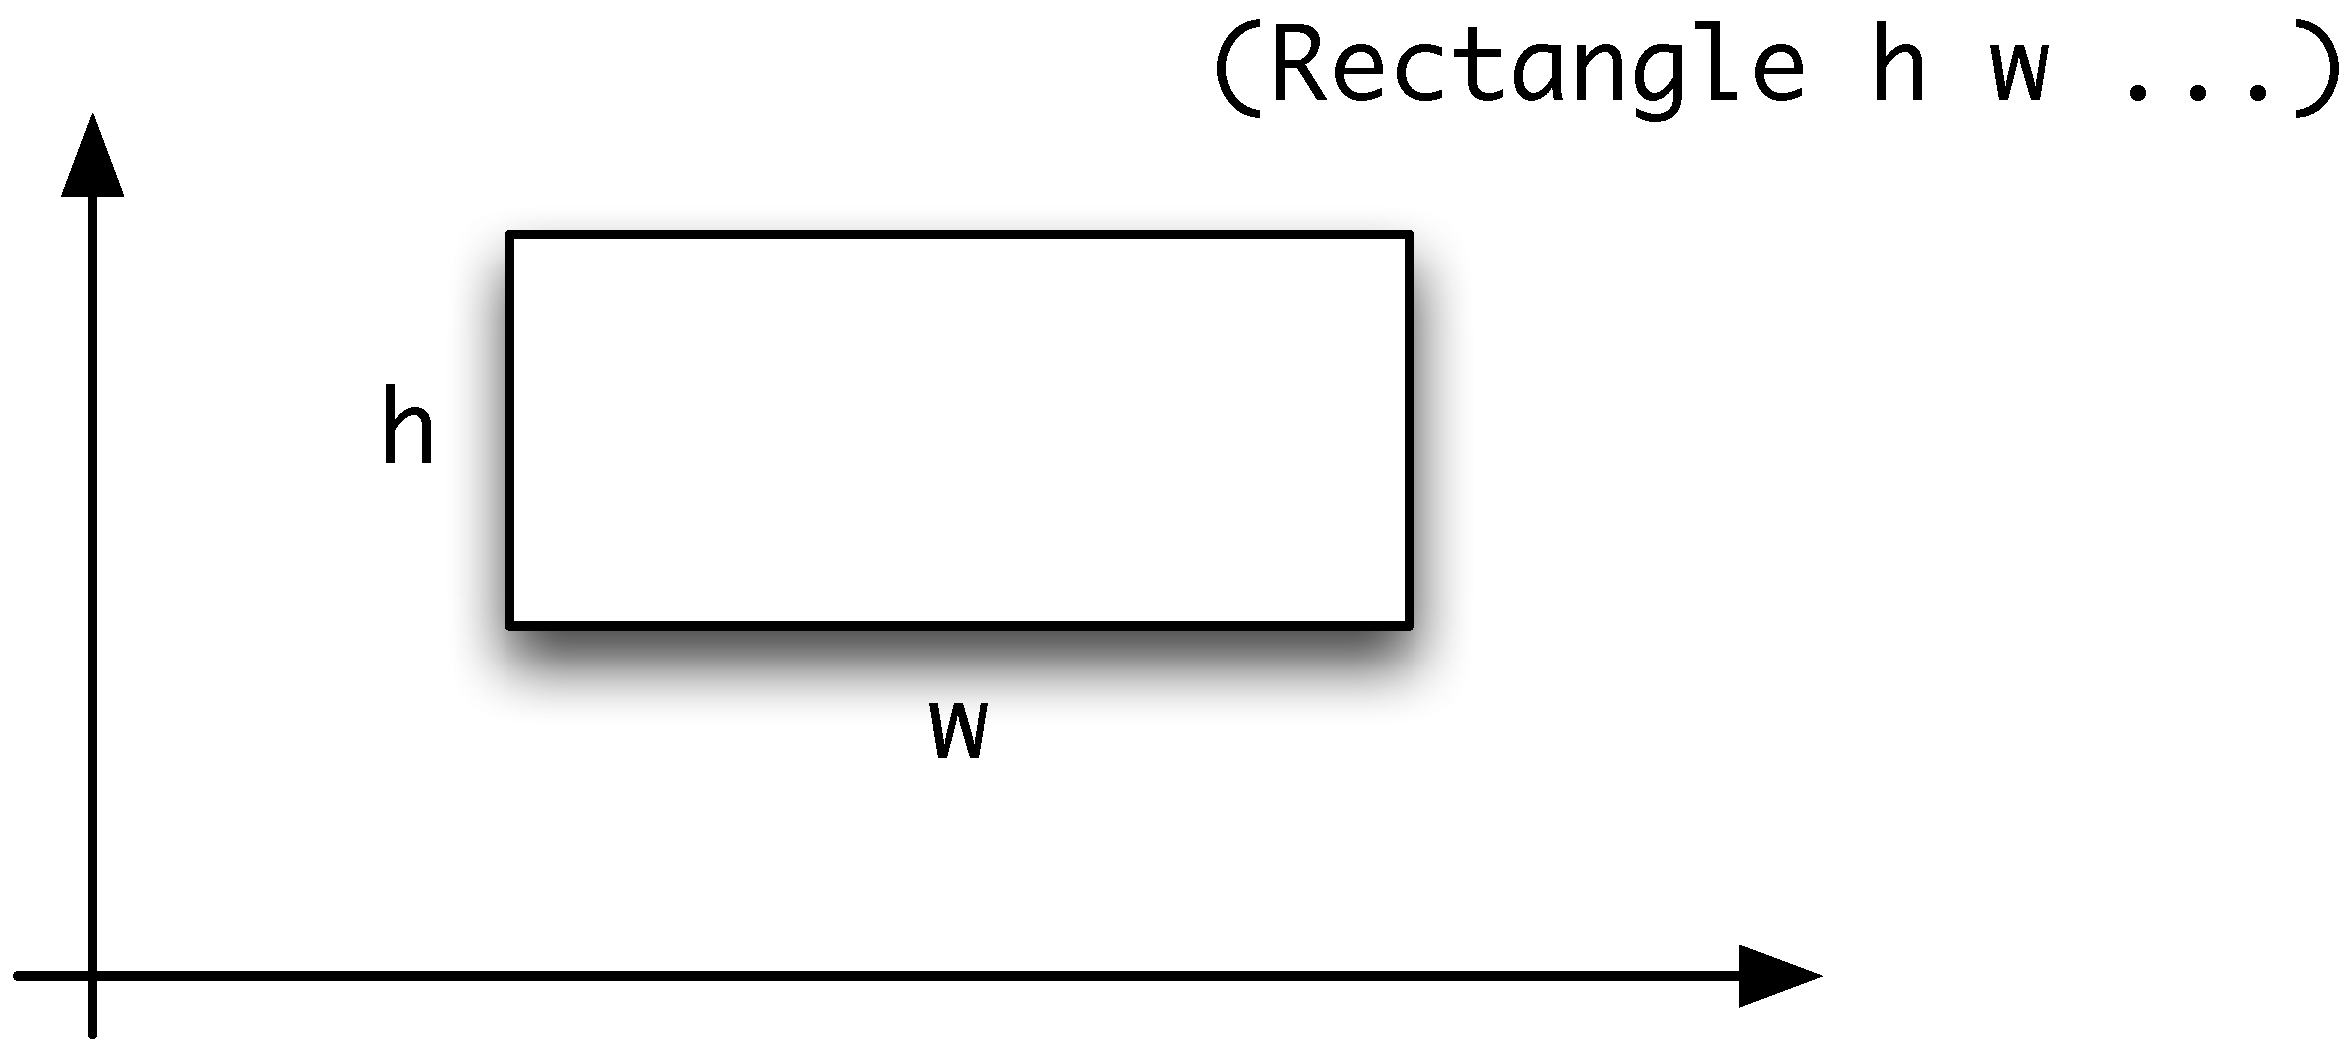
\includegraphics[width=3in]{Pictures/rectanglePos.pdf}
\end{center}

\item
Calling the new shape type \texttt{NewShape}, define a function 
\begin{alltt}
move :: Float -> Float -> NewShape -> NewShape 
\end{alltt}
which moves a shape by the two offsets given:
\begin{center}
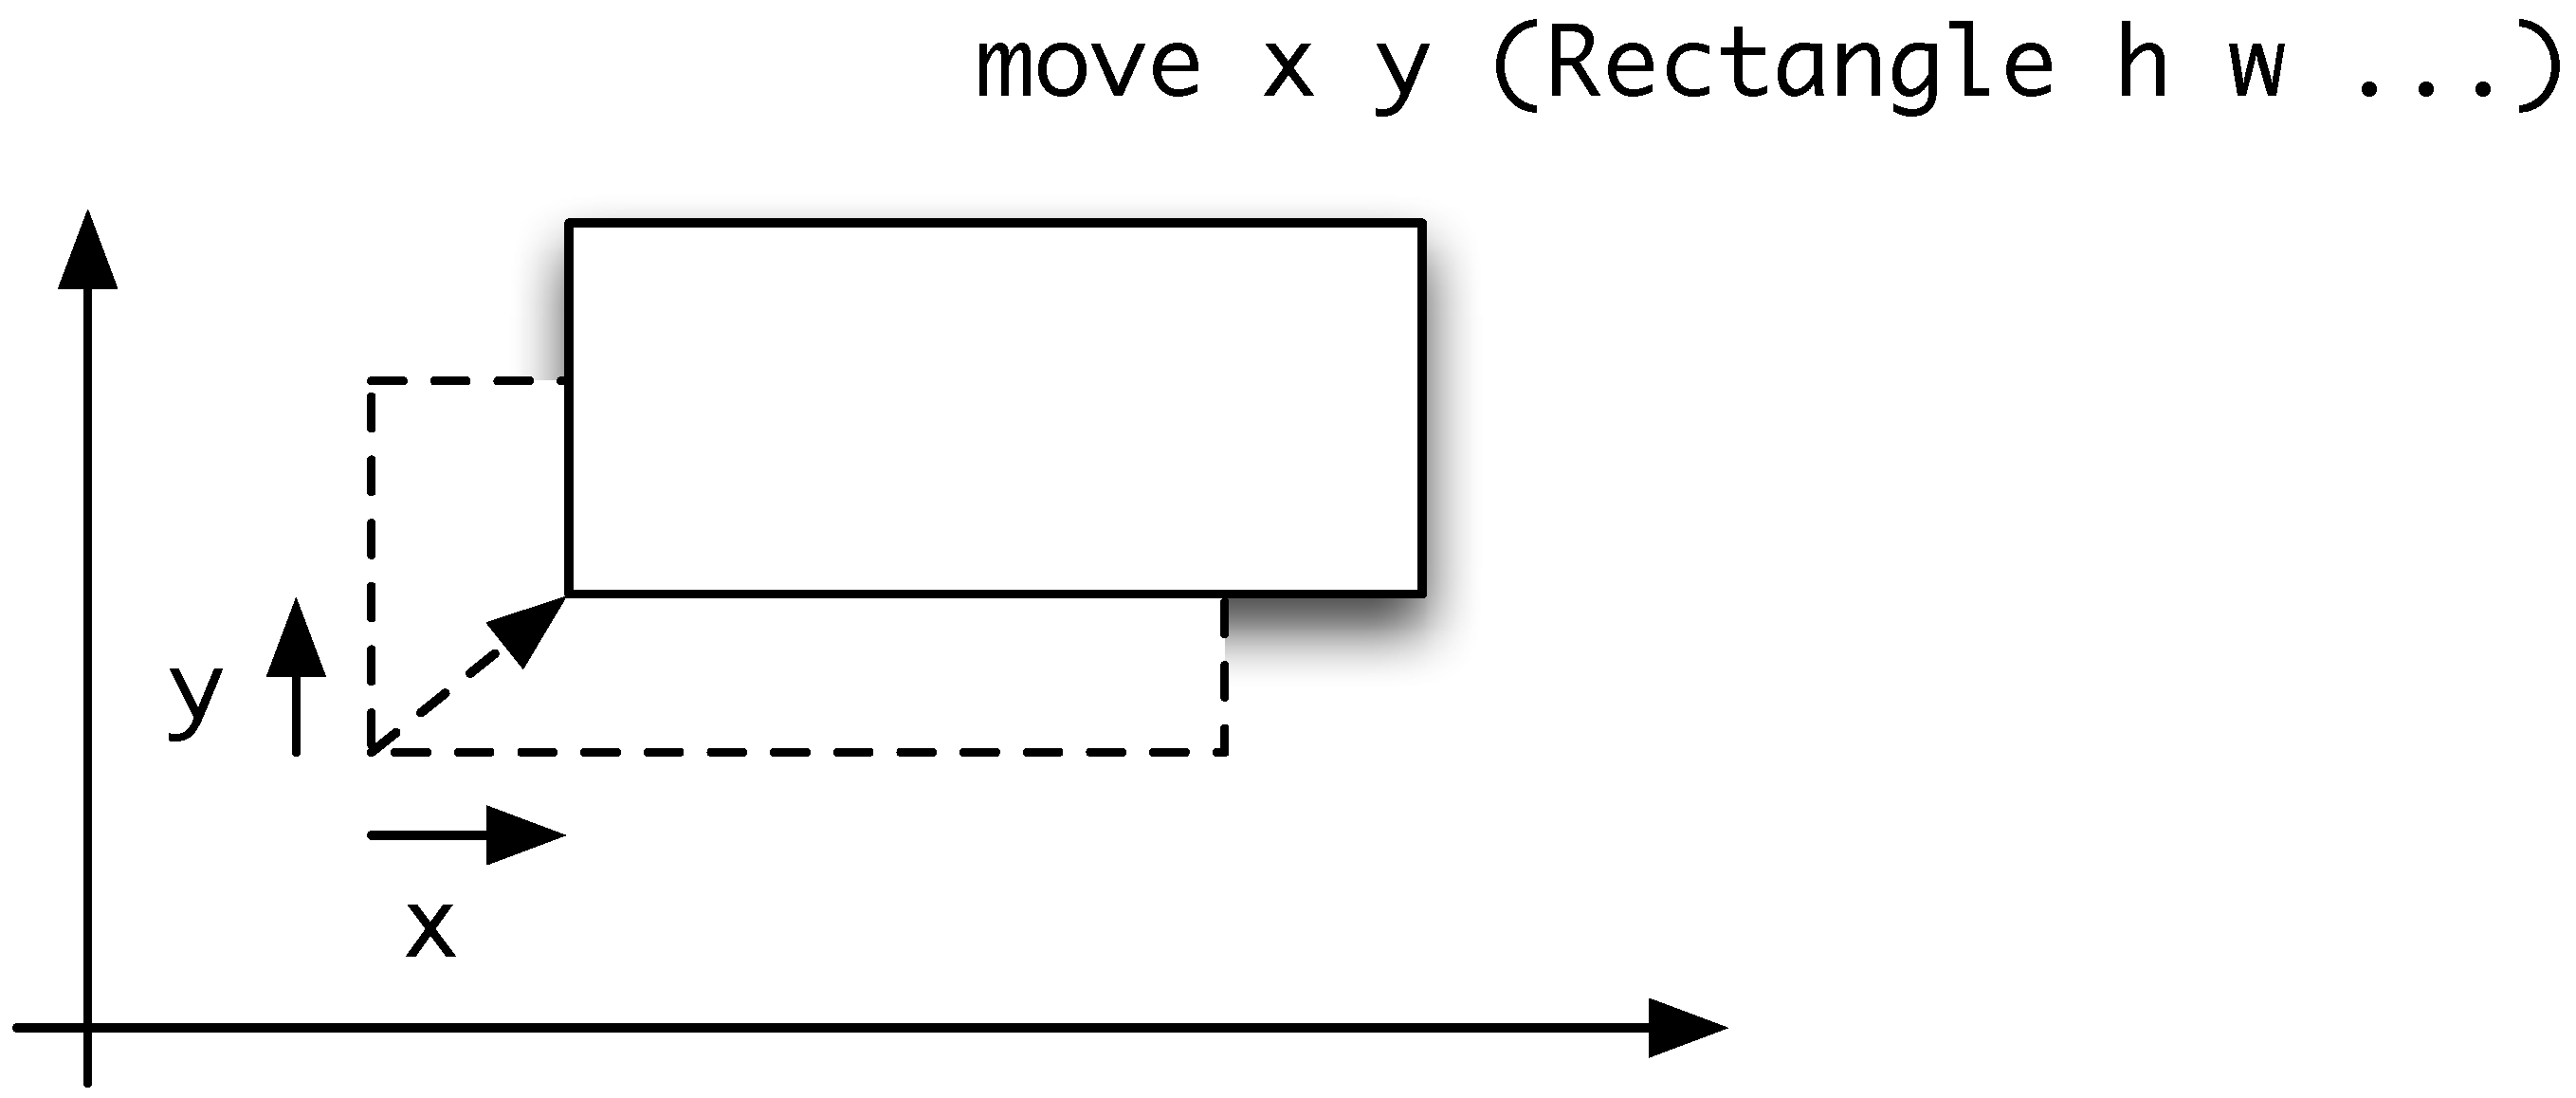
\includegraphics[width=3.5in]{Pictures/rectangleMove.pdf}
\end{center}


\item
Define a function to test whether two \texttt{NewShapes} overlap.

\item
Some houses have a number; others have a name.
How would you implement the type of `strings or numbers' used as a part of an
address? Write a function which gives the textual form of one of these objects. Give a
definition of a type of names and addresses using the type you have defined.


\end{exercises}


\index{algebraic type|)}


\section{Our approach to lists}
\index{lists|(}
\index{lists!approach taken}


Lists are a remarkably expressive data type. We can represent a text as
a list of lines, each of which is a list of words; we can represent a
collection of information, like a supermarket bill, as a list of
individual items of data; we can represent a collection of readings from
a measuring device as a list of \texttt{Floats}, to mention but three
potential applications. 

At the same time, there are many different things which we can
do to lists, some of which first came out in our implementation of \texttt{Pictures}
by lists\minx{Picture}
in Chapter \ref{intro}. Given a list we can split it up according to
various criteria, we can sort it, select items from it and transform all
its members in a particular way. We can combine lists by joining them
together or by coalescing corresponding elements. We can combine all
the members of a list together -- by taking their sum, maximum or
conjunction, say -- among many other operations. 
Haskell contains many built-in list functions
and operators in the standard prelude \texttt{Prelude.hs}\minx{Prelude.hs}
and also various library modules, including
\texttt{List.hs}. \minx{List.hs}

Because Haskell has so many list functions built in, we can approach our discussion of
lists in two very different ways. We could argue that we should start by 
defining list-manipulating functions for ourselves, and only use library
functions after we have understood their definitions.\footnote{This was
essentially the approach taken in the first edition of this book.} On
the other hand, we could adopt a `toolkit' approach, and simply discuss
the library functions and how they can be used. What we aim to do here
is to combine the two approaches, often introducing and using functions
before they are defined explicitly, but then looking `under the bonnet' to see
how these functions are defined  and how we can define other functions
for ourselves. 


In the remainder of this chapter we introduce some of the facilities for
list manipulation within Haskell, particularly \emph{list comprehensions} which give a flexible notation for transforming and selecting elements of lists. This is followed in Chapter \ref{progLists} with an overview of the list functions available to the Haskell programmer, and in Chapter \ref{defFunLists} we see how to define these and
other functions for ourselves.




\section{Lists in Haskell}

A list in Haskell is a collection of items from a given type. For every type \texttt{t}
there is a Haskell type \texttt{[t]} of lists of elements from \texttt{t}.
\begin{alltt}
[1,2,3,4,1,4] :: [Integer]
[True]        :: [Bool]
\end{alltt}
We read these as `\texttt{[1,2,3,4,1,4]} is a list of \texttt{Integer}' and
`\texttt{[True]} is a list of \texttt{Bool}'. \texttt{String} is a synonym
\minx{String}
for {\mi
[Char]} and the two lists which follow are the same.
\begin{alltt}
['a','a','b'] :: String
"aab"         :: String
\end{alltt}
We can build lists of items of any particular type, and so we can have lists of
functions and lists of lists of numbers, as in
\begin{alltt}
[fastFib,fastFib]  :: [ Integer -> Integer ]
[[12,2],[2,12],[]] :: [ [Integer] ]
\end{alltt}
As can be seen, the list with elements \texttt{\eone}, \texttt{\etwo}, \texttt{\subscr{e}{3}}, \texttt{\subscr{e}{4}} and \texttt{\subscr{e}{5}}  is written by enclosing the elements in square brackets, separated by commas, like this
\begin{alltt}
[\texttt{\eone},\texttt{\etwo},\texttt{\subscr{e}{3}},\texttt{\subscr{e}{4}},\texttt{\subscr{e}{5}}]
\end{alltt}
As a special case the empty list, \texttt{[]},\minx{[]} which contains no items, is
an element of every list type.

The order of the
items in a list is significant, as is the number of times that an item
appears. The three lists of numbers which follow are therefore all
different:
\begin{alltt}
[1,2,1,2,2]
[2,1,1,2,2]
[2,1,1,2]
\end{alltt}
The first two have length \texttt{5}, while the third has length
\texttt{4}; the first element of the first list is \texttt{1}, while
the first element of the second is \texttt{2}. A set\index{sets} is another kind of
collection in which the ordering of items and the number of 
occurrences of a particular item are not relevant; we look at sets in Chapter \ref{adt}.

There are some other ways of writing down lists of numbers, characters and other enumerated
types 
\begin{itemize}
\item \texttt{[n ..\ m]} is the list \texttt{[n,n+1,\ldots,m]}; if \minx{..}
\texttt{n} exceeds \texttt{m}, the list is empty.
\begin{alltt}
[2 ..\ 7]     \step{}[2,3,4,5,6,7]
[3.1 ..\ 7.0] \step{}[3.1,4.1,5.1,6.1,7.1]
['a' ..\ 'm'] \step{}"abcdefghijklm"
\end{alltt}
\item \texttt{[n,p ..\ m]} is the list of numbers whose first two elements are \texttt{n} and
\texttt{p} and whose last is \texttt{m}, with the numbers ascending in steps
of \texttt{p-n}. For example,
\begin{alltt}
[7,6 ..\ 3]       \step{}[7,6,5,4,3]
[0.0,0.3 ..\ 1.0] \step{}[0.0,0.3,0.6,0.8999999999999999]
['a','c' ..\ 'n'] \step{}"acegikm"
\end{alltt}
\item In both cases it can be seen that if the step size does not allow us to
reach \texttt{m} exactly, the last item of the list is the element in the
sequence that is closest to \texttt{m}, even if it appears to ``overshoot'' the limit. It can also
be the case that rounding errors on \texttt{Float} lead to lists being
different from what is anticipated; an example is given in the
exercises.
\end{itemize}
In the next section we turn to a powerful method of writing down lists which we can use to define
a variety of list-manipulating functions. 

\subsection*{The \texttt{String} type}
\index{strings|(}
\minx{String}

We first introduced the string type \texttt{String} in Section \ref{char}, and saw there that strings are sequences of characters, that is sequences of \texttt{Char}s. In fact, the \texttt{String} type is a special case of lists, 
\begin{alltt}
type String = [Char]
\end{alltt}
and all the polymorphic prelude functions in Figure \ref{polyListOps}
can be used over strings. We saw in Section \ref{char} how to write
the special characters such as newline and tab using the `escapes'
\texttt{'\bs{n}'} and \texttt{'\bs{t}'}, and also how we could join strings using `\texttt{++}': of course, we can use that operator on \emph{any} list type. 
Other functions over strings can be found in the library \texttt{Data.String}.\minx{Data.String}

%\subsection*{Strings and values}

Built into Haskell are the overloaded functions \texttt{show}\index{show@\texttt{show}}
and \texttt{read}\minx{read}, which convert from a value to a
\texttt{String} and
vice versa; for instance,
\begin{alltt}
show (2+3)           \step{}"5"
show (True || False) \step{}"True"
\end{alltt}
In the opposite direction, the function \texttt{read} is used to convert
a string to the value it represents, so that
\begin{alltt}
read "True" \step{}True
read "3"    \step{}3
\end{alltt}
In some situations it will not be clear what should be the result type
for
\texttt{read} -- it is then possible to give a type to the application,
as in
\begin{alltt}
(read "3") :: Integer
\end{alltt}
the  result of which will be \texttt{3} and its type, \texttt{Integer}. 

We saw in Section \ref{char} that \texttt{show} and \texttt{read} could be used to and from \texttt{String} from other types; a
full explanation of the types of \texttt{read} and \texttt{show} can be
found in Chapter \ref{typeClasses}.
\index{strings|)}


\begin{exercises}

\item
What value has the expression \texttt{[0, 0.1 ..\ 1]}? Check your answer
in GHCi  and explain any discrepancy there might be between the two.

\item
How many items does the list \texttt{[2,3]} contain? How many does \texttt{[[2,3]]}
contain? What is the type of \texttt{[[2,3]]}?

\item
What is the result of evaluating \texttt{[2 ..\ 2]}? What about \texttt{[2,7 ..\ 4]}?
Try evaluating \texttt{[2,2 ..\ 2]}; to \textbf{interrupt evaluation}\index{evaluation!interrupt}
\minx{Ctrl-C} in GHCi under Windows or Unix you
need to type \texttt{Ctrl-C}.
\end{exercises}



\section{List comprehensions}
\label{listComps}
\index{list comprehensions|(}

One of the distinct features of a functional language is the list
comprehension notation, which has no parallels in other paradigms.

In a list comprehension we write down a description of a list in terms
of the elements of another list. From the first list we
\textbf{generate} elements, which we \textbf{test} and
\textbf{transform} to form elements of the result. We will describe 
list comprehensions with a single generator in this section; Section
17.3 covers the general case. Nevertheless, the simple case we
look at here is very useful in writing a variety of list-processing
programs. We introduce the topic by a series of examples.

\begin{example}
\subexample*{1.}
Suppose that the list \texttt{ex} is \texttt{[2,4,7]}, then the list
comprehension
\begin{alltt}
[ 2*n | n<-ex]\hfill (1)
\end{alltt}
will be
\begin{alltt}
[4,8,14]
\end{alltt}
as it contains each of the elements \texttt{n} of the list \texttt{ex}, doubled:
\texttt{2*n}. We can read \texttt{(1)} as saying
\begin{quote}
`Take all \texttt{2*n} where \texttt{n} comes from \texttt{ex}.'
\end{quote}
where the symbol \texttt{<-}\minx{<-} is meant to resemble the mathematical symbol for
being an element, `$\in$'. We can write the evaluation of the list
comprehension in a table, thus:
\begin{alltt}
[ 2*n | n <- [2,4,7] ] 
 
  n   =   2   4   7
2*n   =   4   8  14
\end{alltt}

\subexample*{2.}
In a similar way, 
\begin{alltt}
[ isEven n | n<-ex ] \step{}[True,True,False]
\end{alltt}
if the function \texttt{isEven} has the 
definition
\begin{alltt}
isEven :: Integer -> Bool
isEven n = (n `mod` 2 == 0)
\end{alltt} 
In
list comprehensions \texttt{n<-ex} is called a {\bf generator} because it
\index{list comprehensions!generator}
generates the data from which the results are built. On the left-hand side
of the `\texttt{<-}'\minx{<-}
there is a variable, \texttt{n}, while on the right-hand
side we put the list, in this case \texttt{ex}, from which the elements are taken.


\subexample*{3.}
We can combine a generator with one or more {\bf tests}, 
\index{list comprehensions!test} which are Boolean
expressions, thus:
\begin{alltt}
[ 2*n | n <- ex , isEven n , n>3 ]\hfill (2)
\end{alltt}
\texttt{(2)} is paraphrased as
\begin{quote}
`Take all \texttt{2*n} where \texttt{n} comes from \texttt{ex}, \texttt{n} is even and
greater than \texttt{3}.'
\end{quote}
Again, we can write the evaluation in tabular form.
\begin{alltt}
[ 2*n | n <- [2,4,7] , isEven n , n>3 ]
 
       n   =   2   4   7
isEven n   =   T   T   F
     n>3   =   F   T   
     2*n   =       8   
\end{alltt}
The result of \texttt{(2)} will therefore be the list \texttt{[8]}, as \texttt{4} is
the only even element of \texttt{[2,4,7]} which is greater than \texttt{3}.

\subexample*{4.}
Instead of placing a variable to the left of the arrow `\texttt{<-}', we can put
a pattern. For instance,
\begin{alltt}
addPairs :: [(Integer,Integer)] -> [Integer]\minx{addPairs}
addPairs pairList = [ m+n | (m,n) <- pairList ]
\end{alltt}
Here we choose all the pairs in the list \texttt{pairList}, and add their
components to give a single number in the result list. For example,
\begin{alltt}
[ m+n | (m,n) <- [(2,3),(2,1),(7,8)] ]
 
  m   =   2   2   7  
  n   =   3   1   8
m+n   =   5   3  15
\end{alltt}
giving the result 
\begin{alltt}
addPairs [(2,3),(2,1),(7,8)] \step{}[5,3,15]
\end{alltt}

\subexample*{5.}
We can add tests in such a situation, too:
\begin{alltt}
addOrdPairs :: [(Integer,Integer)] -> [Integer]
addOrdPairs pairList = [ m+n | (m,n) <- pairList , m<n ]
\end{alltt}
so that with the same input example, 
\begin{alltt}
[ m+n | (m,n) <- [(2,3),(2,1),(7,8)] , m<n ]
 
  m   =   2   2   7  
  n   =   3   1   8
m<n   =   T   F   T
m+n   =   5      15
\end{alltt}
giving 
\begin{alltt}
addOrdPairs [(2,3),(2,1),(7,8)] \step{}[5,15]
\end{alltt}
since the second pair in the list, \texttt{(2,1)}, fails the test.

\subexample*{6.}
Note that we can simply test elements, with the
effect that we filter some of the elements of a list, according to a
Boolean condition. To find all the digits in a string we can say
\begin{alltt}
digits :: String -> String\minx{digits}
digits st = [ ch | ch<-st , isDigit ch ] 
\end{alltt}
where the function
\begin{alltt}
isDigit :: Char -> Bool
\end{alltt}
imported from the module \texttt{Data.Char} is \texttt{True} on those characters which are digits: \texttt{'0'},
\texttt{'1'} up to \texttt{'9'}.

\subexample*{7.}
A list comprehension can form a part of a larger function definition.
Suppose that we want to check whether all members of a list of integers
are even, or all are odd. We can write
\begin{alltt}
allEven xs = (xs == [x | x<-xs, isEven x])
allOdd xs  = ([] == [x | x<-xs, isEven x])
\end{alltt}
We will see list comprehensions in practice in the next section when we
examine a simple library database.


\subexample*{8.}
The pattern on the left-hand side of an arrow need not match everything in the list: take the example
\begin{alltt}
totalRadii :: [Shape] -> Float
totalRadii shapes = sum [r | Circle r <- shapes]
\end{alltt}
The effect of this is to match only the circles in the \texttt{shapes} list, and to ignore any other shapes, so that, for example
\begin{alltt}
totalRadii [Circle 2.1, Rectangle 2.1 3.2, Circle 4.7] \step{}6.8
\end{alltt}
This also applies to patterns for built-in types, so we can define
\begin{alltt}
sings :: [[Integer]] -> [Integer]
sings xss = [x | [x] <-xss ]
\end{alltt}
which extracts all singleton elements from a list of lists:
\begin{alltt}
sings [[],[1],[2,3],[4],[5,6,7],[8]] \step{}[1,4,8]
\end{alltt}

\end{example}
\begin{exercises}

\item
Give a definition of a function
\begin{alltt}
doubleAll :: [Integer] -> [Integer]
\end{alltt}
which doubles all the elements of a list of integers.

\item
Give a definition of a function
\begin{alltt}
capitalize :: String -> String
\end{alltt}
which converts all small letters in a \texttt{String}
into capitals, leaving the other characters unchanged. How would you
modify this function to give
\begin{alltt}
capitalizeLetters :: String -> String
\end{alltt}
which behaves in the same way except that all non-letters are
removed from the list? 

\item
Define the function
\begin{alltt}
divisors :: Integer -> [Integer]
\end{alltt}
which returns the list of divisors of a positive integer (and the empty
list for other inputs). For instance,
\begin{alltt}
divisors 12 \step{}[1,2,3,4,6,12]
\end{alltt}
A prime number \texttt{n} is a number whose only divisors are
\texttt{1} and \texttt{n}. Using \texttt{divisors}
or otherwise define a function
\begin{alltt}
isPrime :: Integer -> Bool
\end{alltt}
which checks whether or not a positive integer is prime (and returns
\texttt{False} if its input is not a positive integer).

\item
Define the function
\begin{alltt}
matches :: Integer -> [Integer] -> [Integer]
\end{alltt}
which picks out all occurrences of an integer n in a list. For instance,
\begin{alltt}
matches 1 [1,2,1,4,5,1] \step{}[1,1,1]
matches 1 [2,3,4,6]     \step{}[]
\end{alltt}
Using \texttt{matches} or otherwise, define a function
\begin{alltt}
elem :: Integer -> [Integer] -> Bool
\end{alltt}
which is \texttt{True}
if the \texttt{Integer} is an element of the list, and \texttt{False}
otherwise. For the examples above, we have
\begin{alltt}
elem 1 [1,2,1,4,5,1] \step{}True
elem 1 [2,3,4,6]     \step{}False
\end{alltt}
Since \texttt{elem} is a prelude function, you need to hide it as
described on page \pageref{redefName}.


\item Define a function 
\begin{alltt}
onSeparateLines :: [String] -> String
\end{alltt}
which takes a list of strings and returns a single string which when printed
shows the strings on separate lines.

\item Give a function 
\begin{alltt}
duplicate :: String -> Integer -> String
\end{alltt}
which takes a string and an integer, \texttt{n}. The result is \texttt{n}
copies of the string joined together.
If \texttt{n} is less than or equal to \texttt{0}, the result should be
the empty string, \texttt{""}, and if \texttt{n} is \texttt{1}, the result will be the
string itself.

\item Give a function 
\begin{alltt}
pushRight :: String -> String
\end{alltt}
which takes a string and
forms a string of length \texttt{linelength} by putting spaces at the front of
the
string. If \texttt{linelength} were \texttt{12} then \texttt{pushRight "crocodile"}
would be \texttt{"\ \ \ crocodile"}. How would you make \texttt{linelength}
a parameter of this function?

\item Can you criticize the way the previous function is specified? Look for a
case in which it is not defined what it should do -- it is an exceptional
case.

\item
Define a function 
\begin{alltt}
fibTable :: Integer -> String
\end{alltt}
which produces a table of Fibonacci numbers. For instance, the effect of
\texttt{putStr (fibTable 6)}
should be
\begin{alltt}
        n        fib n
        0            0
        1            1
        2            1
        3            2
        4            3
        5            5
        6            8                
\end{alltt}


\index{list comprehensions|)}
\end{exercises}


\section{A library database}
\label{library}
\index{examples!library database|see{library database}}
\index{library database|(}

This section presents a simple model of the loan data kept by a library,  and
illustrates how list comprehensions are used in practice.

A library uses a database to keep a record of the books on loan to
borrowers; we first look at which type to use to model the database, and
then look at the functions which extract information from a database.
This is followed by a discussion of how to model changes to the database, and we
conclude by exploring how the database functions can be tested.

\subsection*{Types}

In modelling this situation, we first look at the types of the objects
involved. People and books are represented by strings
\begin{alltt}\minx{Person}\minx{Book}
type Person = String
type Book   = String
\end{alltt}
The database can be represented in a number of different ways, including the following four possibilities:
\begin{itemize}
\item We could record each loan as a \texttt{(Person,Book)} pair.
\item We could define a \texttt{data} type for loans, like this:
\begin{alltt}
data Loan = Loan Person Book
\end{alltt}
and then record each loan in the form \texttt{Loan "Alice" "Asterix"}.
\item We could associate with each person the list of books that they
have borrowed, using a pair \texttt{(Person,[Book])}.
\item We could record a list of borrowers with each book, thus:
\texttt{([Person],Book)},
\end{itemize}
Here we choose to
make the database a list of \texttt{(Person,Book)} pairs. If the pair \texttt{("Alice" ,
"Asterix")} is in the list, it means that \texttt{"Alice"} has borrowed the book
called \texttt{"Asterix"}. We therefore define
\begin{alltt} 
type Database = [ (Person , Book) ] \minx{Database}
\end{alltt}
We have chosen this representation because it is simple, and also
treats people and books in the same way, rather than grouping data in an
asymmetrical way.

An example object of this type is
\begin{alltt}
exampleBase :: Database
exampleBase 
= [ ("Alice" , "Tintin")  , ("Anna" , "Little Women") ,
    ("Alice" , "Asterix") , ("Rory" , "Tintin") ]
\end{alltt}
After defining the types of the objects involved, we consider the functions
which work over the database.
\begin{titemize}
\item Given a person, we want to find the book(s) that he or she has borrowed, if any. 
\item Given a book, we want to find the borrower(s) of the book, if any. (It
is assumed that there may be more than one copy of any book.)
\item Given a book, we want to find out whether it is borrowed.
\item Given a person, we may want to find out the number of books that he or she has
borrowed.
\end{titemize}
Each of these {\bf lookup} functions will take a \texttt{Database}, and a 
\texttt{Person} or \texttt{Book}, and return the result of the query. Their types will be
\begin{alltt}
books       :: Database -> Person -> [Book]\minx{books}
borrowers   :: Database -> Book -> [Person]\minx{borrowers}
borrowed    :: Database -> Book -> Bool\minx{borrowed}
numBorrowed :: Database -> Person -> Int\minx{numBorrowed}
\end{alltt}
Note that \texttt{borrowers} and \texttt{books} return lists; these can contain
zero, one or more items, and so in particular an empty list can signal that a book has no
borrowers, or that a person has no books on loan.

Two other functions need to be defined. We need to be able to model a book being loaned to 
a person and a loaned book being returned. The functions modelling these
will take a
database, plus the loan information, and return a {\em different\/} database,
which is the original with the loan added or removed. These {\bf update}
functions will have type
\begin{alltt}
makeLoan   :: Database -> Person -> Book -> Database\minx{makeLoan}
returnLoan :: Database -> Person -> Book -> Database\minx{returnLoan}
\end{alltt}

\subsection*{Defining the lookup functions}

We concentrate on the definition of the function 
\minx{books}
\begin{alltt}
books :: Database -> Person -> [Book]\minx{books}
\end{alltt}
which forms a model for the other lookup functions. For the \texttt{exampleBase}, we have
\begin{alltt}
books exampleBase "Alice" = [ "Tintin" , "Asterix" ]
books exampleBase "Rory"  = [ "Tintin" ]
\end{alltt}
How are these found? In the \texttt{"Alice"} case we need to run through the 
list \texttt{exampleBase} finding all the pairs whose first component is
\texttt{"Alice"}; for each of these we return the second component. As a
list comprehension, we have
\begin{alltt}\index{list comprehensions!library database}
[ book | (person,book) <- exampleBase , person=="Alice" ]

person       =   "Alice"    "Anna"           "Alice"     "Rory"
  book       =   "Tintin"   "Little Women"   "Asterix"   "Tintin"
(person==    =      T          F                T           F 
 "Alice")
  book       =   "Tintin"                    "Asterix"           
\end{alltt}
We make this into a general function by saying
\begin{alltt}
books       :: Database -> Person -> [Book]\minx{books}\hfill(books.1)
books dBase findPerson
  = [ book | (person,book) <- dBase , person==findPerson ]
\end{alltt}
Note that in this definition \texttt{Person} is a type while
\texttt{person} is a variable of type \texttt{Person}.

As we said at the start, \texttt{books} forms a model for the other lookup
functions, which we leave as an exercise. 

\begin{figure}[t]
\beware{Variables in list comprehensions}{\index{pitfalls!list comprehensions}%
\index{list comprehensions!pitfalls}%
There is an important pitfall to do with the
behaviour of variables in list comprehensions. The definition \texttt{(books.1)}
of \texttt{books} above
might appear to be over-complicated. We might imagine that we could say
\begin{alltt}
books dBase findPerson\\\minx{books}
  = [ book | (findPerson,book) <- dBase ]\hfill(books.2)
\end{alltt}
The effect of this is to return all the books borrowed by \emph{all} borrowers,
not just the particular borrower \texttt{findPerson}. 

The reason for this is that the
\texttt{findPerson} in \texttt{(findPerson,book)} is a \emph{new} variable, and not the
variable on the left-hand side of the definition, so in fact \texttt{(books.2)} has
the same effect as
\begin{alltt}
books dBase findPerson = [ book | (new,book) <- dBase ]
\end{alltt}
where it is clear that there is no constraint on the value of \texttt{new} to be
equal to \texttt{findPerson}.
} % end beware
\end{figure}

\subsection*{Defining the update functions}

The database is modified, or updated, by the functions \texttt{makeLoan}
and
\texttt{returnLoan}.
Making a loan is done by adding a pair to the database, which can be done
simply by adding an extra pair to the front of the list of pairs.
\begin{alltt}
makeLoan   :: Database -> Person -> Book -> Database\minx{makeLoan}
makeLoan dBase pers bk = [ (pers,bk) ] ++ dBase
\end{alltt}
We have used the \texttt{++}\minx{++} operator here to join two
lists, namely 
the one element list \texttt{[(pers,bk)]} and the `old' database
\texttt{dBase}.

To return a loan, we need to check through the database, and to remove the
pair \texttt{(pers,bk)}. We therefore run through all the pairs in the
database, and retain those which are not equal to \texttt{(pers,bk)}, thus
\begin{alltt}
returnLoan   :: Database -> Person -> Book -> Database\minx{returnLoan}
returnLoan dBase pers bk
  = [ pair | pair <- dBase , pair /= (pers,bk) ]
\end{alltt}
Note that we have used a simple variable \texttt{pair} rather than a
pattern to run over the pairs in the \texttt{dBase}. This is because we
do not need to deal with the components separately; all we do is check
whether the whole pair is equal to the pair \texttt{(pers,bk)}. On the
other hand we could use a pattern thus:
\begin{alltt}
[ (p,b) | (p,b) <- dBase , (p,b) /= (pers,bk) ]
\end{alltt}
and get exactly the same result.

As we have defined it, the \texttt{returnLoan} function will remove {\em
all\/} pairs \texttt{(pers,bk)} from the database. We will return to
this point in the exercises in Section 9.3.


\subsection*{Testing}
\index{testing!library database}

A Haskell interpreter
acts like a calculator, and this is useful when we wish to test
functions like those in the library database. Any function can be tested by
typing expressions to the GHCi prompt. For example,
\begin{alltt}
makeLoan [] "Alice" "Rotten Romans"
\end{alltt}
To test more substantial examples, it is sensible to put test data into a
script, so we might include the definition of \texttt{exampleBase} as well as
various tests
\begin{alltt}
test1 :: Bool
test1 = borrowed exampleBase "Asterix"

test2 :: Database
test2 = makeLoan exampleBase "Alice" "Rotten Romans"
\end{alltt}
and so on. Adding them to the script means that we can repeatedly evaluate them
without having to type them out in full each time. Another device which can
help is to use \texttt{it},\minx{it}
which is short for `the last expression evaluated' in GHCi.
The following sequence makes a loan, then another, then returns the first.
\begin{alltt}
makeLoan exampleBase "Alice" "Rotten Romans"
makeLoan it "Rory" "Godzilla"
returnLoan it "Alice" "Rotten Romans"
\end{alltt}
To make the tests repeatable it is possible to define a sequence of \texttt{Database} values, and to describe as HUnit tests using these database values. We leave that as an exercise for the reader.

\subsection*{Testing in QuickCheck}
\index{QuickCheck!library database}

We can use QuickCheck to test the database, too. The \texttt{Chapter5} module has a number of properties, but here we include two basic ones:
\begin{itemize}
\item
If we loan \texttt{bk} to \texttt{pers} and then lookup the books loaned to \texttt{pers}, then \texttt{bk} should be in that list:
\begin{alltt}\minx{prop\_db*}
prop_db1 :: Database -> Person -> Book -> Bool

prop_db1 dBase pers bk =
    elem bk loanedAfterLoan == True
         where
           afterLoan = makeLoan dBase pers bk
           loanedAfterLoan = books afterLoan pers
\end{alltt}
\item
If we return the loan of \texttt{bk} to \texttt{pers} and then lookup the books loaned to \texttt{pers}, then \texttt{bk} should be \emph{not} in that list:
\begin{alltt}
prop_db2 :: Database -> Person -> Book -> Bool

prop_db2 dBase pers bk =
    elem bk loanedAfterReturn == False
         where
           afterReturn = returnLoan dBase pers bk
           loanedAfterReturn = books afterReturn pers
\end{alltt}
\end{itemize}

\begin{exercises}
\item
Go through the calculation of
\begin{alltt}
books exampleBase "Charlie" 
books exampleBase "Rory"
\end{alltt}

\item
Define the functions \texttt{borrowers},
\texttt{borrowed} and \texttt{numBorrowed}. To define
\texttt{numBorrowed} you will probably need the
\texttt{length}\minx{length}
function which returns the length of a list.

\item
Give calculations of  
\begin{alltt}
returnLoan exampleBase "Alice" "Asterix"
returnLoan exampleBase "Alice" "Little Women"
\end{alltt}


\item
How would you have to modify the database functions if you had used the type
\begin{alltt}
data Loan = Loan Person Book
\end{alltt}
to model individual loans, rather than the tuple type?

\item
How would you express this as a QuickCheck property: \begin{quote}``Suppose that a particular \texttt{bk} is \emph{not} loaned to a \texttt{pers}. Now make a random loan of \texttt{bk2} to \texttt{pers2}. \texttt{bk} should still not be loaned to \texttt{pers}.''\end{quote}
Would you expect this property to hold? If so, why? If not, why not, and how would you modify it so that it does hold?


\item
Discuss how you would implement the database functions had you used
the representation \texttt{[(Person,[Book])]} rather than
\texttt{[(Person,Book)]}for the database.

\item
How would the tests for the database have to be modified to work with the implementation defined in the previous question? Would the QuickCheck properties have to be modified: if so, how? If not, why not?


\item
Define functions to give more readable output from the database
operations of this section.


\index{library database|)}
\index{lists|)}
\end{exercises}











\begin{summary}
This chapter has introduced the structured types of tuples and lists,
and explained their differences: in a given tuple type, 
\texttt{(\tone,...\tn)}
the elements all have the same form, namely \texttt{(\vone,...\vn)},
with each component \texttt{\subscr{v}{i}} being a member of the corresponding
type \texttt{\subscr{t}{i}}. The list type \texttt{[t]} on the other hand contains
elements \texttt{[\eone,...,\subscr{e}{n}]} of different lengths but in which 
all the values \texttt{\subscr{e}{i}} have the same
type \texttt{t}.

Over tuples we introduced the notion of pattern matching -- in which a
pattern such as \texttt{(x,y)}
could be used to stand for an arbitrary member of a pair type -- and saw
how this led to more readable definitions.

We also saw how we could define our own \texttt{data} types to model product types -- like tuples -- and sums, which can represent types containing a number of different alternative elements.

The bulk of the chapter was an account of the facilities which
Haskell provides for working with lists. These include
various ways of writing lists of elements of base type, including ranges
like \texttt{[2,4..12]}, and \emph{list comprehensions}, in which the members of a list are
generated, tested and transformed from the elements of another list, as
exemplified by
\begin{alltt}
[ toUpper ch | ch <- string , isAlpha ch ]
\end{alltt}
which selects the alphabetic characters from a \texttt{string}, and
converts them to upper case, using functions imported from the module \texttt{Data.Char}. We also saw that \texttt{String} is the list type \texttt{[Char]}.

In the chapters to come we will use the list functions given here in making
our own definitions, as well as finding out about the prelude and library functions for lists, and how they are
themselves defined.
\end{summary}
%\end{document}
